\documentclass[12pt]{article}
%--------------------   start of the 'preamble'
%
\usepackage{graphicx,amssymb,amstext,amsmath,color}
\usepackage[margin=2cm]{geometry}
\usepackage{abstract}
\usepackage{setspace}
\usepackage[footnotesize,bf]{caption}

% TABLE
\usepackage{multicol,hhline,colortbl,multirow}
\usepackage{braket}
\usepackage{siunitx}
\usepackage{hyperref}
\usepackage{authblk}
\usepackage{siunitx}
\usepackage{mathrsfs}
%%\usepackage[sort&compress]{natbib}
%%\bibpunct{(}{)}{,}{a}{, }{;}
%
\usepackage[sort&compress]{natbib}
\bibpunct{[}{]}{,}{s}{}{;}


\definecolor{gray}{gray}{0.8}
\def\mobunits{\square\centi\meter\per\volt\per\second}
\def\gcm{\gram\per\cubic\centi\meter}
\def\ccg{\cellcolor{gray}}

\renewcommand{\labelitemii}{$\circ$}
\renewcommand{\bibname}{References}


\title{MorphCT - testSimple Device Simulations}
\author{Matthew Jones}
\date{\today}

\begin{document}
\maketitle


\section{Test System}

Since the previous deviceKMC summary, we've decided to cut down on the complexity of the morphology and see if we can get sensible results.
The new device morphology is 3x3x3, with the middle vertical slice 100\% mixed phase, and an alternating checkerboard pattern of donor and acceptor on the top and bottom.
A schematic of the device is shown in figure~\ref{fig:device}, where each slice is shown along the X-Z plane, and Y-slices are shown next to each other, separated by pipes.


\begin{figure}[h!]\centering
	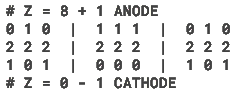
\includegraphics[width=0.3\textwidth]{Figures/device.png}
    \caption{The new testSimple device morphology.}
	\label{fig:device}
\end{figure}


\section{Device Moieties}

In an attempt to fix the device simulation problems, I wanted to remove as many variables as possible from the simulation.
To accomplish this, I think it's important that each device moiety has an identical simulation volume size. This should reduce any problems arising from carriers hopping across boundaries into different sized boxes.
Therefore, I have used opv\_cg to generate molecular morphologies of realistic density for P3HT, PCBM and a mix of the two.
All systems have a box length $l_{x}$ = 10 nm.


Below, I consider the KMCOut outputs for each.


\begin{center}
\begin{tabular}{| c | c | c | c | c | c | c |}
\hline
\rule{0pt}{2.5ex} 
\multirow{2}{*}{\textbf{Simulation}}&\multirow{2}{*}{\textbf{Carrier}}&\textbf{Density}&\textbf{Anisotropy}&\textbf{Anisotropy}&\textbf{Mobility}&\textbf{Intra-}\\
                            &&(\SI{}{\gcm})&(Arb. U.)&(Shape)&(\SI{}{\mobunits})&\textbf{\%}\\
\hhline{|=======|}
\textbf{Neat P3HT}&\rule{0pt}{2.5ex}Hole&1.1&0.0009&Spherical&1.99$\times 10^{0}$&--\%\\
\ccg\textbf{Neat PCBM}&\ccg \rule{0pt}{2.5ex}Electron&\ccg 1.5&\ccg 0.0046&\ccg Spherical&\ccg 2.20$\times 10^{-3}$&\ccg --\%\\
\multirow{2}{*}{\textbf{P3HT/PCBM Mix}}&\rule{0pt}{2.5ex}Hole&\multirow{2}{*}{1.3}&0.0220&Spherical&1.15$\times 10^{0}$&--\%\\
&\ccg \rule{0pt}{2.5ex}Electron&&\ccg 0.0018&\ccg Spherical&\ccg 1.90$\times 10^{-6}$&\ccg --\%\\
\hhline{-------}
\end{tabular}\label{table:mob}
\captionof{table}{MorphCT calculated mobilities for each structural moiety in the testSimple device.}
\end{center}


\begin{itemize}
    \item{\textcolor{red}{As a first note, these jobs were run before the issues with the atom size were reconciled in the REU UA forcefield.
                As such, the CA atoms in the thiophene rings are not treated as being the same size as the FCA atoms in the fullerenes, even though they should be the same.
                In these systems, $\sigma = 3.905$, $r_{CT} = r_{FCT} = 1.0 \sigma$ but $r_{CA} = 0.9 \sigma$ and $r_{FCA} = 0.784 \sigma$.
        This will need fixing before publication, but the idea here is to get the device simulations working so for now we can carry on.}}
    \item{There are several interesting things going on here.}
    \item{P3HT:
            \begin{itemize}
                \item{The anisotropy is very spherical, which is characteristic of a disordered morphology.}
                \item{This rings true - the morphology looks disordered (see figure~\ref{fig:morphologies}).
                    The system was equilibrated at a temperature of T = 3.0, which we would expect to be ordered, however that is clearly not the case.}
                \item{Annoyingly, the recorded mobility is very high - on a par with that of an ordered, structured morphology.}
                \item{This is very confusing, but I'm currently running jobs at a state point we know to be ordered and I'll try and work out what's going on after that instead.}
                \item{\textcolor{blue}{Note to self: A good thing to compare here could be the diffraction pattern.
                    Looking at the differences between the 10nm sisordered and ordered P3HT, as well as the original p1 P3HT morphologies that we published on might be elucidating.}}
                \item{Otherwise, the difference between the pristine film and the mix is pretty negligible.}
            \end{itemize}
    }
    \item{PCBM:
            \begin{itemize}
                \item{The neat film looks good. Spherical transport, reasonable mobility - the hallmarks of things going well.}
                \item{The electron transport in the mix is terrible, however. 
                        We've suddently lost 3 orders of magnitude of mobility compared to the pristine film.
                    This warrants investigation.}
            \end{itemize}
        }
\end{itemize}


\begin{figure}[h!]\centering
	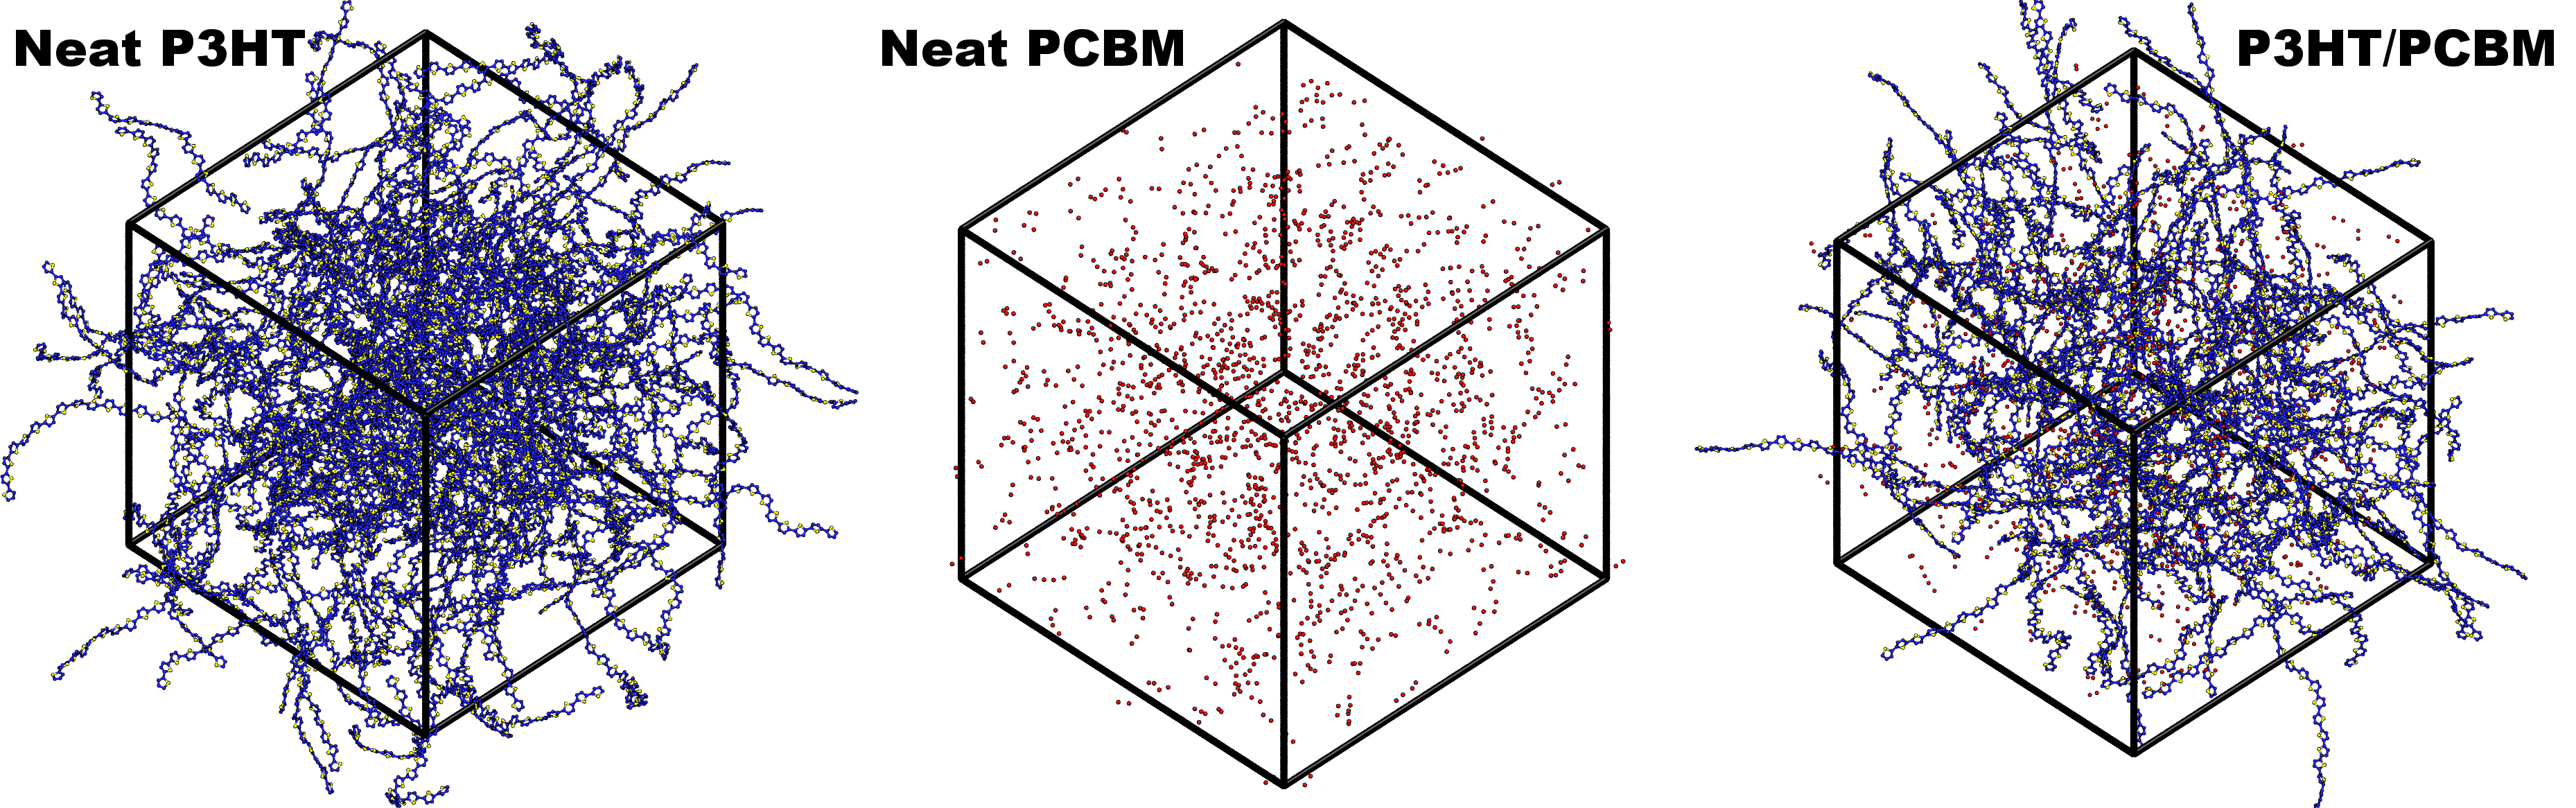
\includegraphics[width=\textwidth]{Figures/morphologies.png}
    \caption{The three morphologies used in this investigation. 
    For clarity, only the S and CA atoms corresponding to the thiophene ring are shown in the P3HT chains, and only the O atoms are shown for the PCBM molecules to help show where functionalization aggregation is occuring in the morphology.}
	\label{fig:morphologies}
\end{figure}


\section{Mean Squared Displacements}


\begin{figure}[h!]\centering
	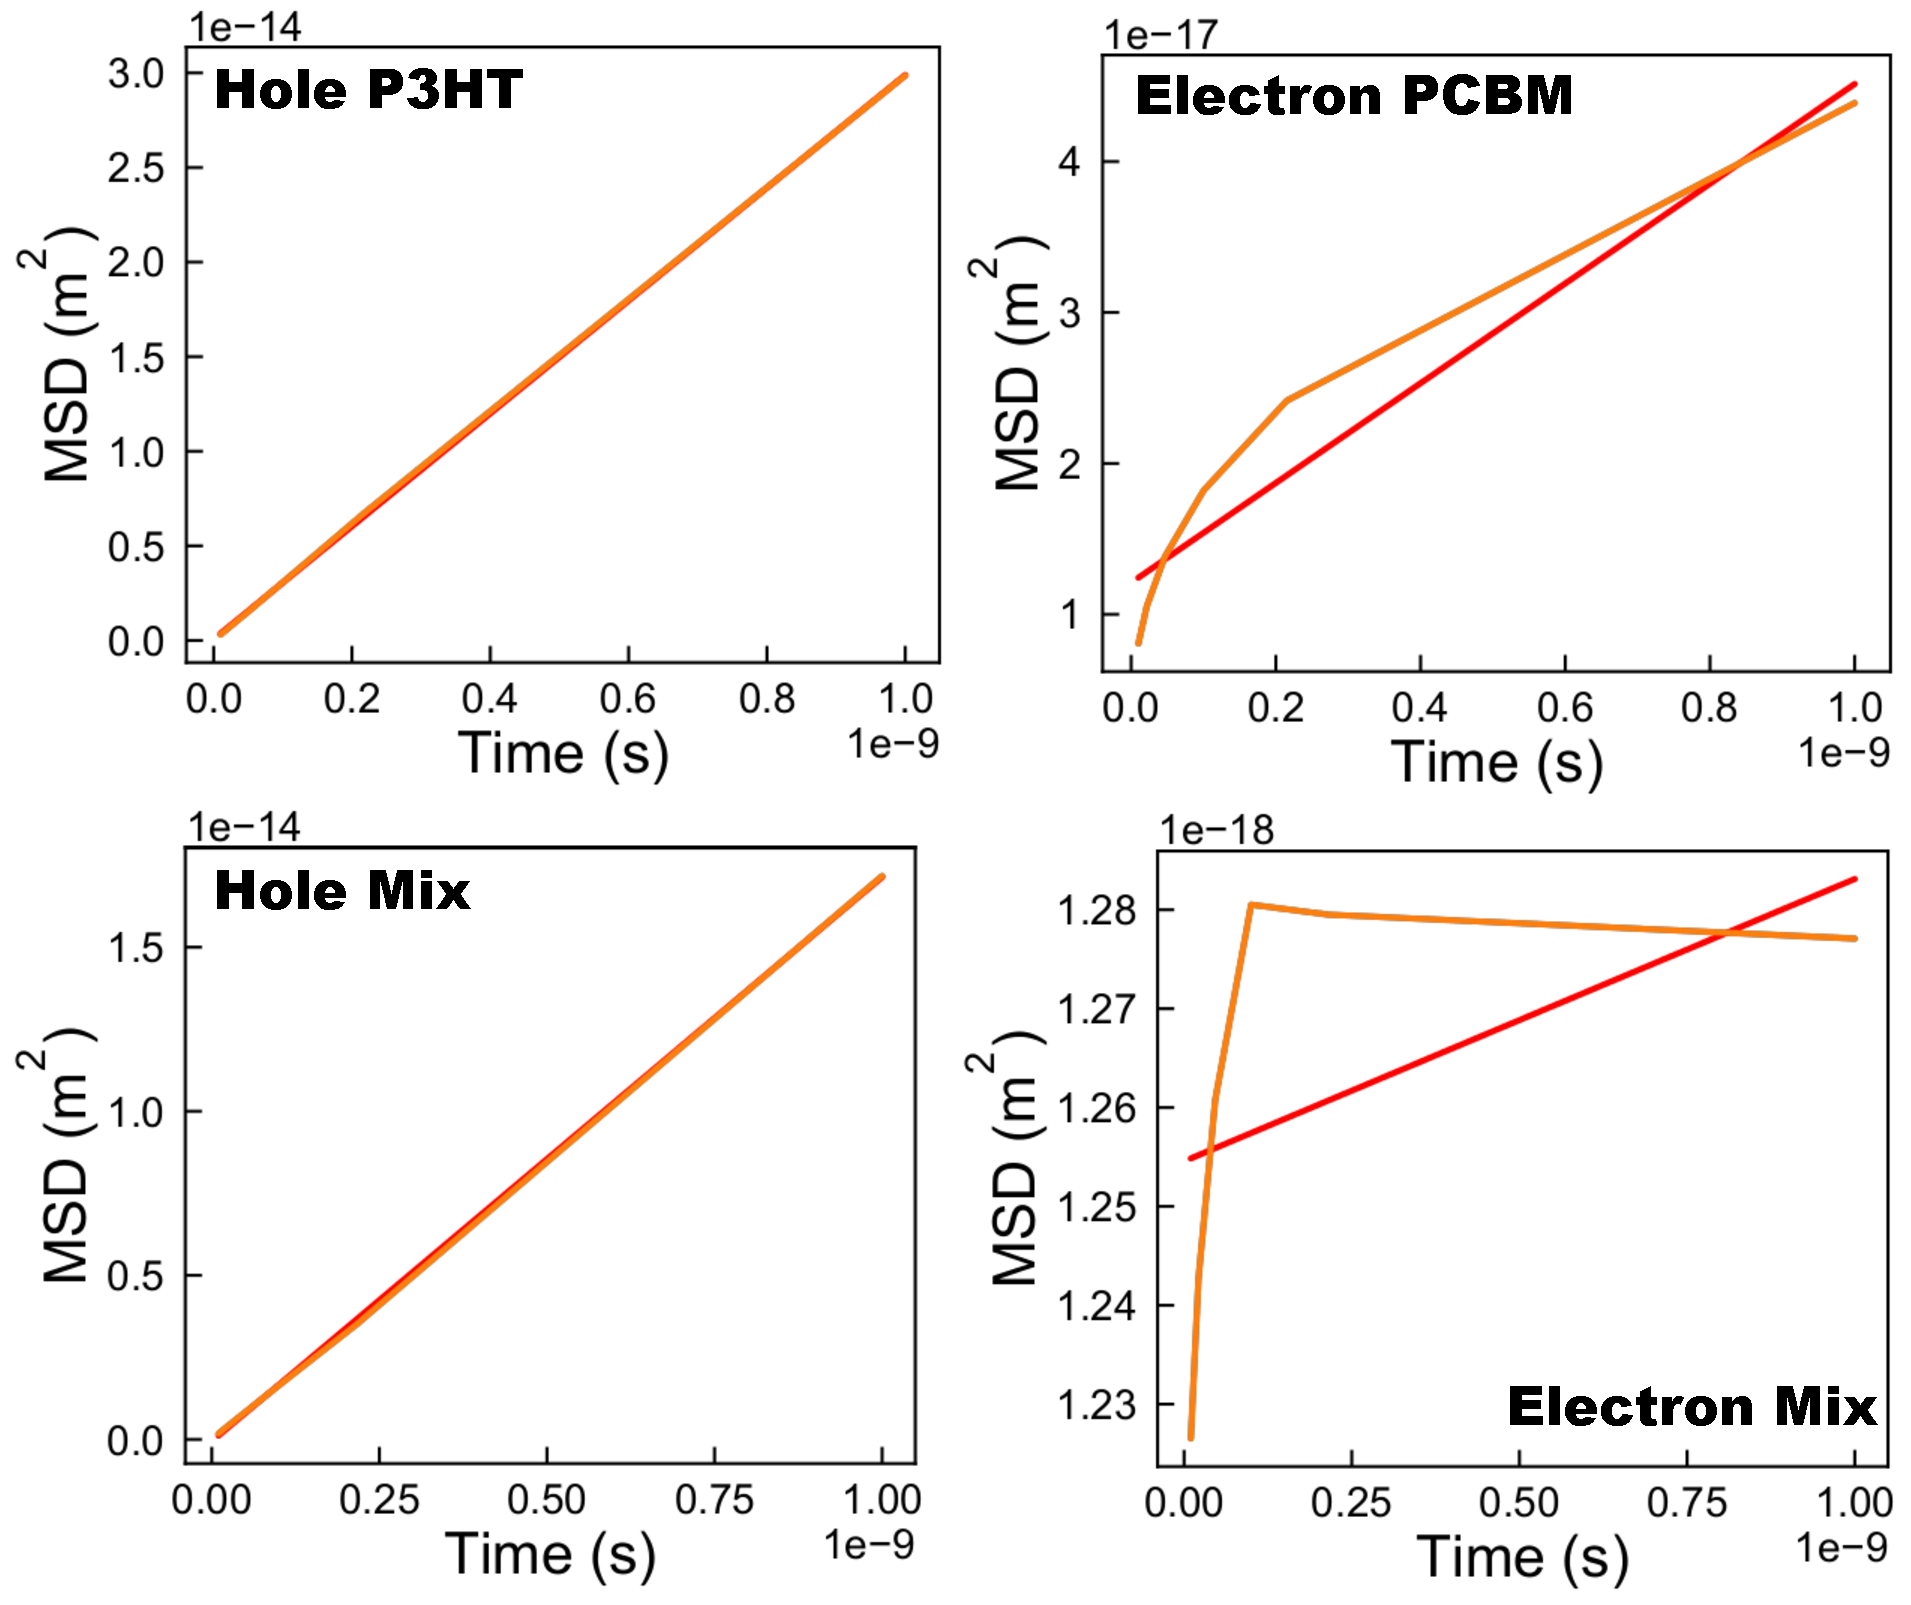
\includegraphics[width=\textwidth]{Figures/MSD.pdf}
    \caption{The mean squared displacement fits for each carrier type in the investigated morphologies.
    The orange line is the simulated KMC data.
    The red line describes the least-squared best linear fit, the gradient of which is taken to be the diffusion coefficient.}
	\label{fig:MSD}
\end{figure}


Figure~\ref{fig:MSD} shows the best linear fits to the MSD for each of the carriers simulated in the KMC.
In both cases, the hole fits are excellent, with an $r^{2} > 99.99$\%.
The same cannot be said about the electron fits, however.
Even though the electron mobility in the pristine PCBM film made sense, it seems as if the MSD is steadily saturating as we noticed with the original p1 P3HT simulations.
The pristine film has a linear fit with $r^{2} = 96.56$\%, whereas the mix has an electron MSD fit of only $r^{2} = 45.92$\%, which is awful.
We need to look at the network information to see the reason why the MSD is so bad.


\clearpage

\section{3D Network and Anisotropy}


\begin{figure}[h!]\centering
	\includegraphics[width=\textwidth]{Figures/3DNetwork.pdf}
    \caption{The plot of the 3D network within one periodic volume of the simulated morphologies.
    Here, nodes correspond to chromophores and vertices are paths taken by carriers within the simulation.
    The colour of the vertex is assigned according to how many hops were counted along that path during the simulation.
    Hops across periodic boundaries are omitted for clarity.}
	\label{fig:network}
\end{figure}


\begin{figure}[h!]\centering
	\includegraphics[width=\textwidth]{Figures/Anisotropy.pdf}
    \caption{The plot of the 3D carrier termination locations.
        Here, each data point corresponds to the location of a carrier (which started in the origin periodic box) when the KMC simulation time was reached.
    It therefore shows the anisotropy of the transport, as well as giving an idea of how far carriers travelled during the simulation.
    }
	\label{fig:anisotropy}
\end{figure}


It is clear from figure~\ref{fig:network} that the P3HT is very well interconnected compared to the PCBM in all morphologies.
In fact, the PCBM systems are so poorly calculated that carrier motion either becomes throttled due to a very small number of routes out of the periodic simulation box (in the case of Neat PCBM), or indeed become completely trapped such that the electron's only option is to hop between the same two or three molecules, saturating the MSD and leading to very low mobilities.
The anisotropy graphs also bear out this hypothesis - the holes are permitted to move $\sim$ 100 nm in the longest simulations, whereas the electrons are confined to nearby simulation volumes ($\sim$ 10 nm in the case of neat PCBM) or are completely locked into the initial volume ($\sim$ 4 nm in the case of the Mix).


\textcolor{red}{Exploration of the RDF (not shown) has suggested a possible solution to this issue.
In P3HT, chromophore centres-of-mass are located around 3~\AA~from each other.
As such, to prevent having to calculate hundreds of thousands of transfer integrals for chromophore pairs which would never be selected by KMC, an artifical hopping cut-off of 1 nm was instigated.
However, when considering `small' molecules such as PCBM and the perylene derivative DBP, 1 nm away from the chromophore centre-of-mass is still located on the same molecule.
It is therefore no longer appropriate to set the cut-off to 1 nm.
The location of the minimum between the second- and third-nearest-neighbour peaks in the PCBM RDF was found to be around 4$\sigma$, corresponding to a distance of 1.6 nm.
Therefore, leaving the hole hopping-distance cut-off as 1 nm and changing the electron hopping-distance cut-off to 2 nm might be sufficient to bolster the network and give more realistic MSDs.}

\textcolor{red}{Theoretically, the only limit to this methodology is computational.
    That is, if we were to set a maximum hopping distance of the box-length, our mobility characteristics should be unaffacted - providing we are not in the regime described above where the hopping cut-off is too low.
    It stands to reason that the longest hops will have the lowest transfer integrals and not be selected as often by KMC anyway.
However, an extremely large cut-off like this would dramatically increase the number of ORCA calculations to be performed, significantly increasing total computation time.
}

\textcolor{red}{I am now re-running the PCBM-containing systems with the increased electron hopping-distance cut-off to 2 nm to see how the results are affected.}
\textcolor{blue}{Additionally, I am rerunning all of the structures again using opv\_cg, this time with the most up-to-date atom sizes according to Evan's work on the resultant diffraction patterns.
    Finally, the P3HT system is being run at a different state-point in order to try and promote ordered chain stacking.
The results from this P3HT system might be able to elucidate why the disordered P3HT chains are able to produce such high mobilities, despite the high paracrystallinity.}


\clearpage

\section{Searching for ordered P3HT chains}

The P3HT-containing jobs I ran over the weekend with the improved forcefield and the following parameters:
\begin{itemize}
    \item{$\phi$ = 0.9}
    \item{$T$ = 3.5}
    \item{$\epsilon$ = 0.8}
\end{itemize}
did not result in ordered $\pi$-stacked chains as anticipated.
The above parameters were selected because Evan's clustering criteria were satisfied more frequently for these systems, resulting in larger clusters in the morphology - usually an indication of better ordering.


\begin{figure}[h!]\centering
    \begin{tabular}{cc}
        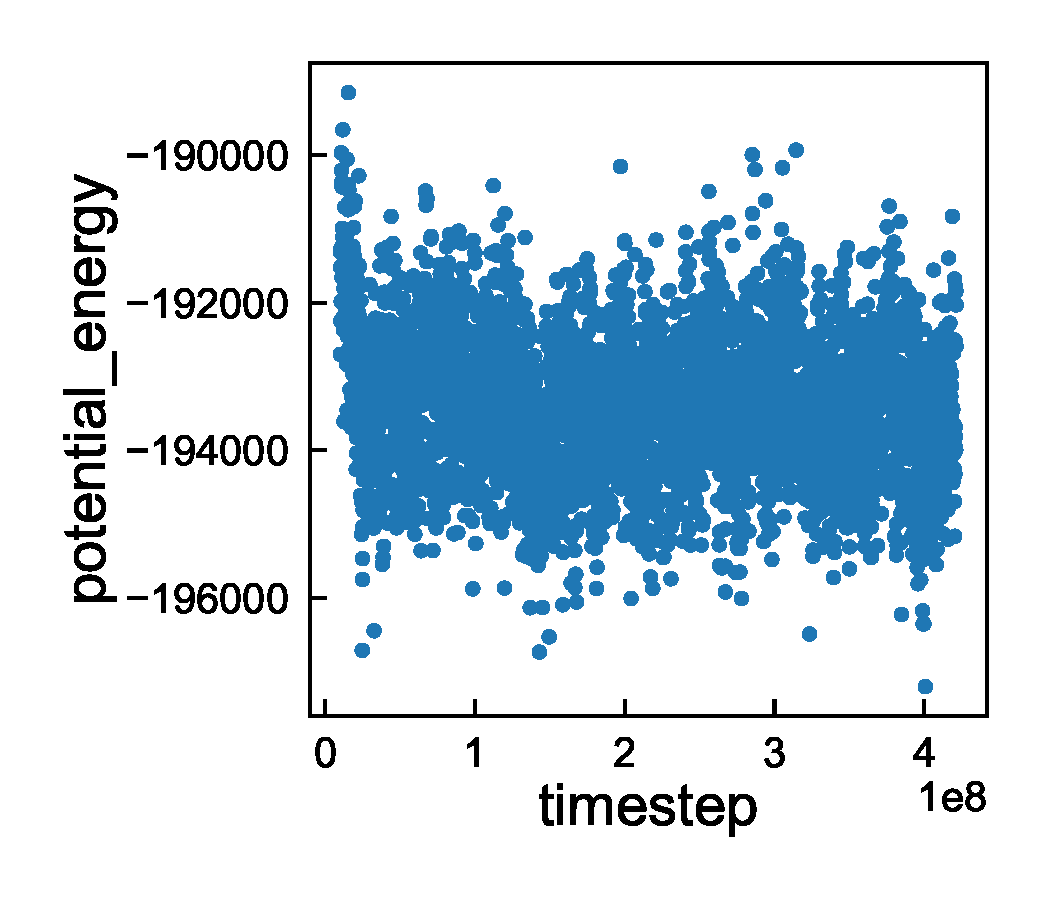
\includegraphics[width=0.5\textwidth]{Figures/P3HTPE.pdf}&
	    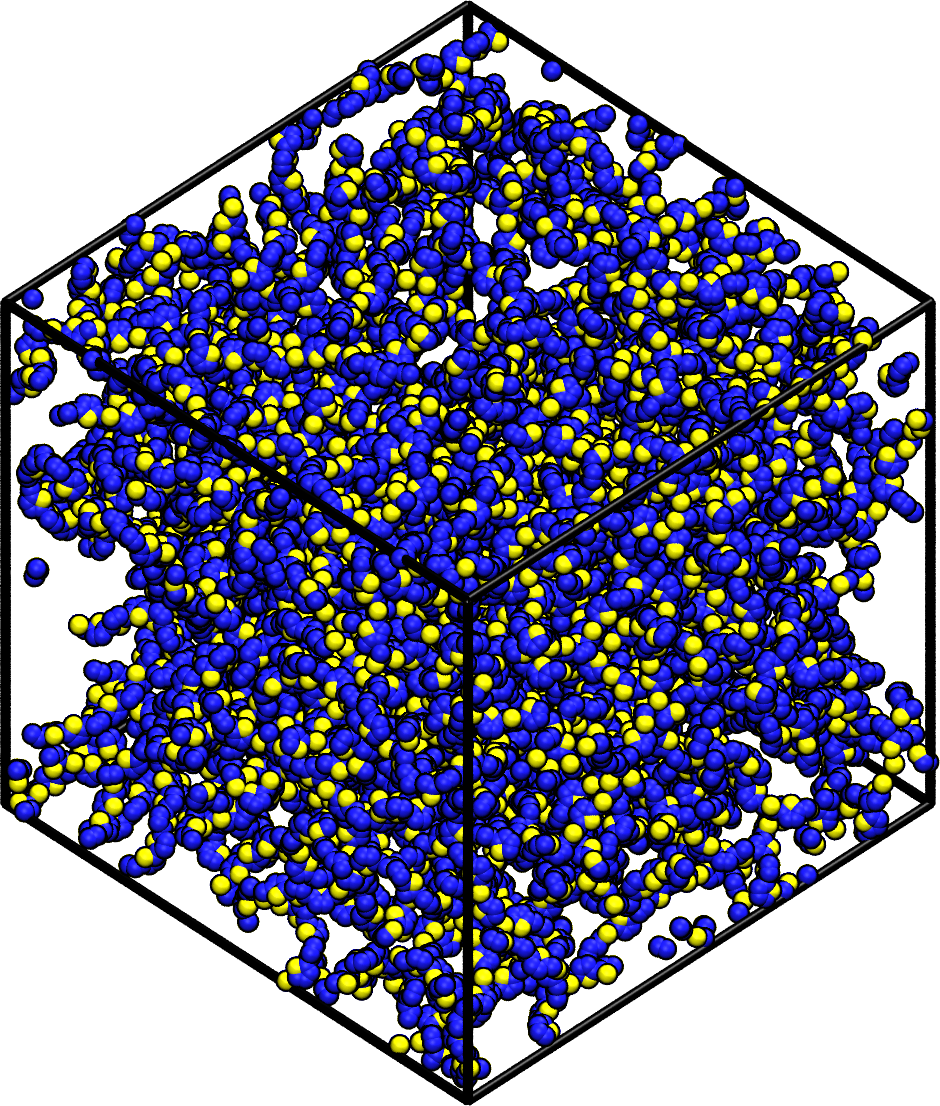
\includegraphics[width=0.5\textwidth]{Figures/P3HTMorph.png}
    \end{tabular}
    \caption{The Neat P3HT system. Left: The potential energy evolution over the 96 hour simulation, with the first hundred datapoints removed. Right: The resultant morphology. Only the thiophene rings are shown for clarity.}
	\label{fig:P3HTPE}
\end{figure}


The Neat P3HT system, containing 265 chains was rerun using the above parameters for 96 hours.
Figure~\ref{fig:P3HTPE}a shows that the morphology appears to have equilibrated in this time, however, the resultant morphology is still disordered (Figure~\ref{fig:P3HTPE}b).
This is unusual, since other systems with different numbers of molecules have shown the correct $\pi$-stacking at this statepoint, and the PE does not appear to be evolving in this case.


\begin{figure}[h!]\centering
    \begin{tabular}{cc}
        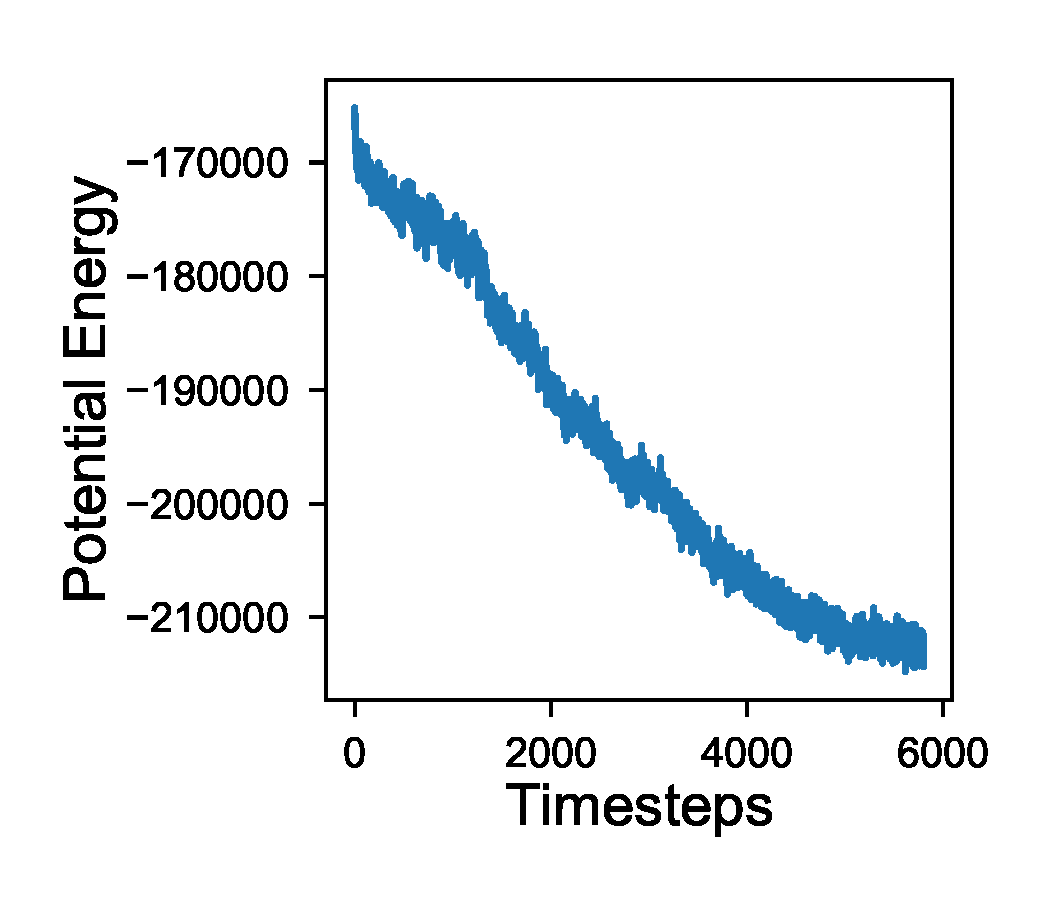
\includegraphics[width=0.5\textwidth]{Figures/P3HT500.pdf}&
	    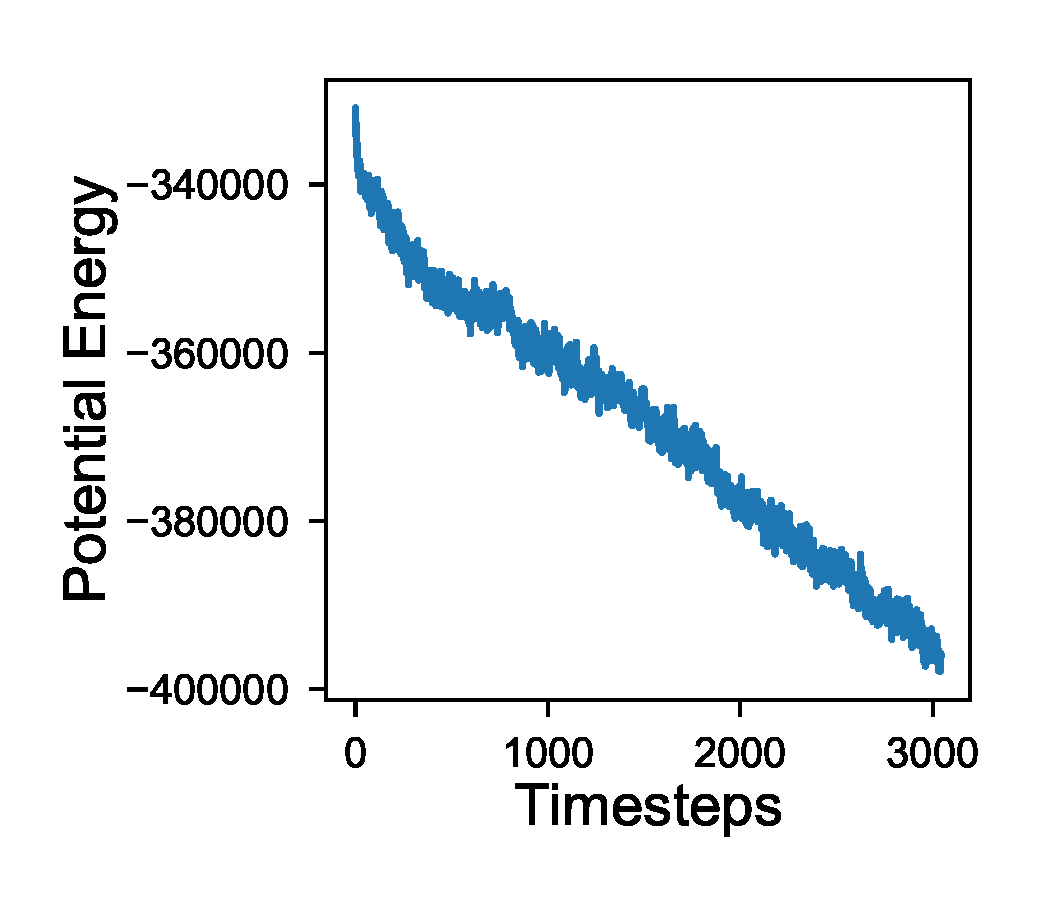
\includegraphics[width=0.5\textwidth]{Figures/P3HT1000.pdf}
    \end{tabular}
    \caption{Potential energy evolution for Evan's 500-molecule P3HT system (left) and for 1000 molecules (right).
    The X-axis is in units of 1E5 timesteps, so the total simulation runtimes are comparable to the current data.
    Note that these simulations are not quick the same statepoint as the current work, as they were run at T = 4.0, whereas the current work was run at T = 3.5.}
	\label{fig:P3HTPEs}
\end{figure}


A useful comparison here is the absolute value of the pair-potential energy in energy units per molecule between this and the ordered P3HT systems.
This should give some idea of how far away the system shown in~\ref{fig:P3HTPE} is, in terms of free energy, from forming the $\pi$ stacks.
Figure~\ref{fig:P3HTPEs} shows the evolution in the LJ pair potential energy as a function of simulation time for systems containing 500 and 1000 molecules.
It is clear that the shapes of the curves are quite different to the current system.
The simulations were run at slightly higher temperatures (T = 4.0), but otherwise the same statepoint.
The P3HT model is slightly different to the one used in the current work - the thiophene carbon sigma is 3.8~\AA~in Figure~\ref{fig:P3HTPEs} instead of the 3.1~\AA~used now.


\begin{center}
\begin{tabular}{| c | c | c | c | c |}
\hline
\rule{0pt}{2.5ex} 
\textbf{Number Of Molecules}&\textbf{LJ PE at Eql}&\textbf{LJ PE/mol at Eql}&\textbf{Temp}&\textbf{Carbon Size}\\
\hhline{|=====|}
\ccg 265&\ccg \rule{0pt}{2.5ex}-92755&\ccg -350.02&\ccg 3.5&\ccg 3.1~\AA\\
500&\rule{0pt}{2.5ex}-212478&-424.96&4.0&3.8~\AA\\
\ccg 1000&\ccg \rule{0pt}{2.5ex}-396115&\ccg -396.12&\ccg4.0&\ccg3.8~\AA\\
\hhline{-----}
\end{tabular}\label{table:PE}
\captionof{table}{The potential energy at equilibration for the current system (265 molecules) and the previous two Neat P3HT systems run by Evan (500 and 1000 molecules).
All energies are given in energy units, which are consistent between the three simulations.}
\end{center}

\bibliography{refs}
\bibliographystyle{unsrt}


\end{document}
